\documentclass[11pt]{article}
    \title{\textbf{Tetrahedral mesh orthogonality optimization for solving diffusive problem with finite volume solver}}
    \author{Moie Rousseau}
    \date{}
    
    \addtolength{\topmargin}{-3cm}
    \addtolength{\textheight}{3cm}
    
\usepackage{amsmath}
\usepackage{hyperref}
\usepackage{graphicx}


\begin{document}

\maketitle
\thispagestyle{empty}

\section*{Abstract}

TODO

\section{Introduction}


The finite volume method (FVM) is a classical numerical method to solve complex engineering problem governed by conservation equations such as encountered in computational fluid dynamic \cite{}, heat transfert \cite{}, oil and gas recovery \cite{}, or hydrogeology \cite{}.
The method relies on a discretized representation of the computational domain (the mesh) on which the governing equations of the system are integrated on mesh elements for cell centered scheme or on a control volume for node center scheme, which are latter converted into surface integral across the boundary by the the use of the Gauss theorem \cite{}. %https://www.sciencedirect.com/science/article/pii/B978012849894100007Xare
Using appropriate discretization method for the gradient and laplacian operator \cite{}, the discretization process lead to a set of algebraic equations linking the variable of interest to their neighboring value, which can be solve to obtain the solution to the problem.

In this study, the discretization of the diffusion operator was analysed for cell centered scheme on which a single unknown is associated within each mesh element.
One of the approach to discretize the diffusion term is the classical Two Point Flux Approximation method (TFPA) which consists in approximating the gradient at each face of mesh element using the value associated at both elements sharing the face \cite{moukalled_finite_2016, ferziger_computational_2020}.
This method possesses the appealing properties to be X and Y \cite{}. %TODO
It is also used by a number of research and industrial codes such as Fluent \cite{}, OpenFOAM \cite{} PFLOTRAN \cite{hammond_pflotran_2012}, DuMux \cite{koch_dumux_2021}, PorePy \cite{keilegavlen_porepy_2021}, Open Porous Media flow simulation \cite{rasmussen_the_2021} or Waiwera \cite{} among others. %https://waiwera.readthedocs.io/en/latest/setup_mesh.html
However, for the TPFA method to be accurate, the mesh is required to be orthogonal, i.e. the vector linking the two cell centers must be parallel to the normal of the face shared by the two cells.
If not, the approximation would introduce a $\mathcal{O}(1)$ error which cannot be avoided \cite{}.

Preservation of the appealing properties of the TPFA discretization thus move the difficulty in generating a orthogonal mesh.
Such mesh for arbitrary computational domain can be generated using polygonal Voronoï grid, which by construction, create face orthogonal to the vector linking the two cell centers.
However, such polyhedral mesh are often not conformal and relie on clipping to fit the modeled domain.
Recent research provide quasi-conformal Voronoi meshes by minimizing the volume of cells empassing a 2D feature \cite{merland_voronoi_2014} or by placing seeds such as no clipping is required \cite{abdelkader_vorocrust_2020}.

In the other hand, conformal tetrahedral meshes are easy to generate and often directly integrated within computer-aided engineering (CAE) softwares.
It also exists a variety of reference codes available such as Gmsh \cite{geuzaine_gmsh_2007}, TetGen \cite{si_tetgen_2015}, NETGEN \cite{schoberl_netgen_1997}, CGAL \cite{}, which are now capable of generating billion of elements in an order of minute \cite{hextrem}.
Despite these advantages, they don't respect the orthogonality condition.

Nevertheless, non-orthogonal meshes such as tetrahedral can still be used along with a appropriated correction such as the deferred correction approach \cite{jasak_error_1996, moukalled_finite_2016, ferziger_computational_2020}.
The deferred correction is required where the non-orthogonality of the computational mesh is above 5° \cite{}. %https://www.sciencedirect.com/science/article/pii/S0029549317300596 (see for cell center)
Mesh orthogonality: normal scalar cell center vector superior to 1/3 is good %file:///tmp/mozilla_moise0/MeshQuality-Appendix-A.pdf
openfoam: slow convergence for mesh orthogonality above 80° %https://www.sciencedirect.com/science/article/pii/S0029549317300596 (see for cell center)
They look for orthogonality: 
%https://www.sciencedirect.com/science/article/pii/S0360544215009068?casa_token=2XncBO8cC2EAAAAA:2ElyHYXlp_7U6AfgEwTn-F8ZWls7tZbjbetgQ6Cm00bxm20JBejOxlf4Go2EnBZUhaajeYneAQ#bib22
%https://pdfs.semanticscholar.org/1d52/a4f30ed56bb82791c283eba37d15eee582cd.pdf
%https://sci-hub.wf/10.1051/e3sconf/20171401027
However, the more the mesh is non-orthogonal, the more iteration it will takes + error \cite{traore_robust_2009}. %it's a guess here, so I need to find reference
This therefore suggests that lowering mesh non-orthogonality could increase convergence of the deferred correction, thus saving time and computational ressource.
Up to date, however, it


Variational approach to mesh orthogonality

This study presents an approach for optimizing the tetrahedral mesh orthogonality in order to reduce numerical simulation error and computational time.
Approach is decribed and tested for several mesh and diffusive problem.
Calculation made with OpenFOAM.


see %10.13140/RG.2.2.25688.39681



\section{Mesh optimization}


\subsection{Formulation of optimization problem}

Fully tetrahedral mesh.

The objective of the optimization was to minimize, for each face, the angle between the face normal and the vector connecting the two cells center sharing the considered face by moving the mesh vertices. 
Therefore, the objective function to minimize was defined as follow:
%
\begin{equation}
\begin{aligned}
& \underset{P}{\text{minimize}}
& & c(P) = \sum_{f \in faces} w_f E_f \left( r_f^T \cdot n_f \right)  \\
& \text{subject to}
& & r_f^T \cdot n_f \geq 0, \\
\end{aligned}
\label{eq:opt_problem}
\end{equation}
$r_f$ is the unit vector in the direction connecting the two cell center sharing the considering face $f$ and $n_f$ the unit face normal (Figure \ref{}), and thus the dot product measures the face non-orthogonality.
$E_f$ is the individual face error function which can be used to apply weighting on the face non-orthogonality, for example to penalize high non-orthogonality error versus low error.
The optimization variables $P$ represent the set of mesh points $P_i$ not lying on the boundary %TODO. 
%The dot product give the cosinus of the face normal - cell center vector angle which is maximal when both vector are aligned (i.e. the mesh orthogonal at this face). 
The $w_f$ is a user specified weighting constant factor which allowed give higher importance to some connections compared to other.
Minimizing $c$ therefore contributes to decrease the overall non-orthogonality error of the mesh.

This optimization problem constitute a high dimensional problem, while 3D tetrahedral meshes nowaday contains at several thousands of points, and up to billion sometimes \cite{neau_massively_2020}.
The optimization was thus takled using a gradient-based approach to take advantage of the existence of the objective function derivative (see below) and reduce computation time.

\begin{figure}[h!]
  \centering
  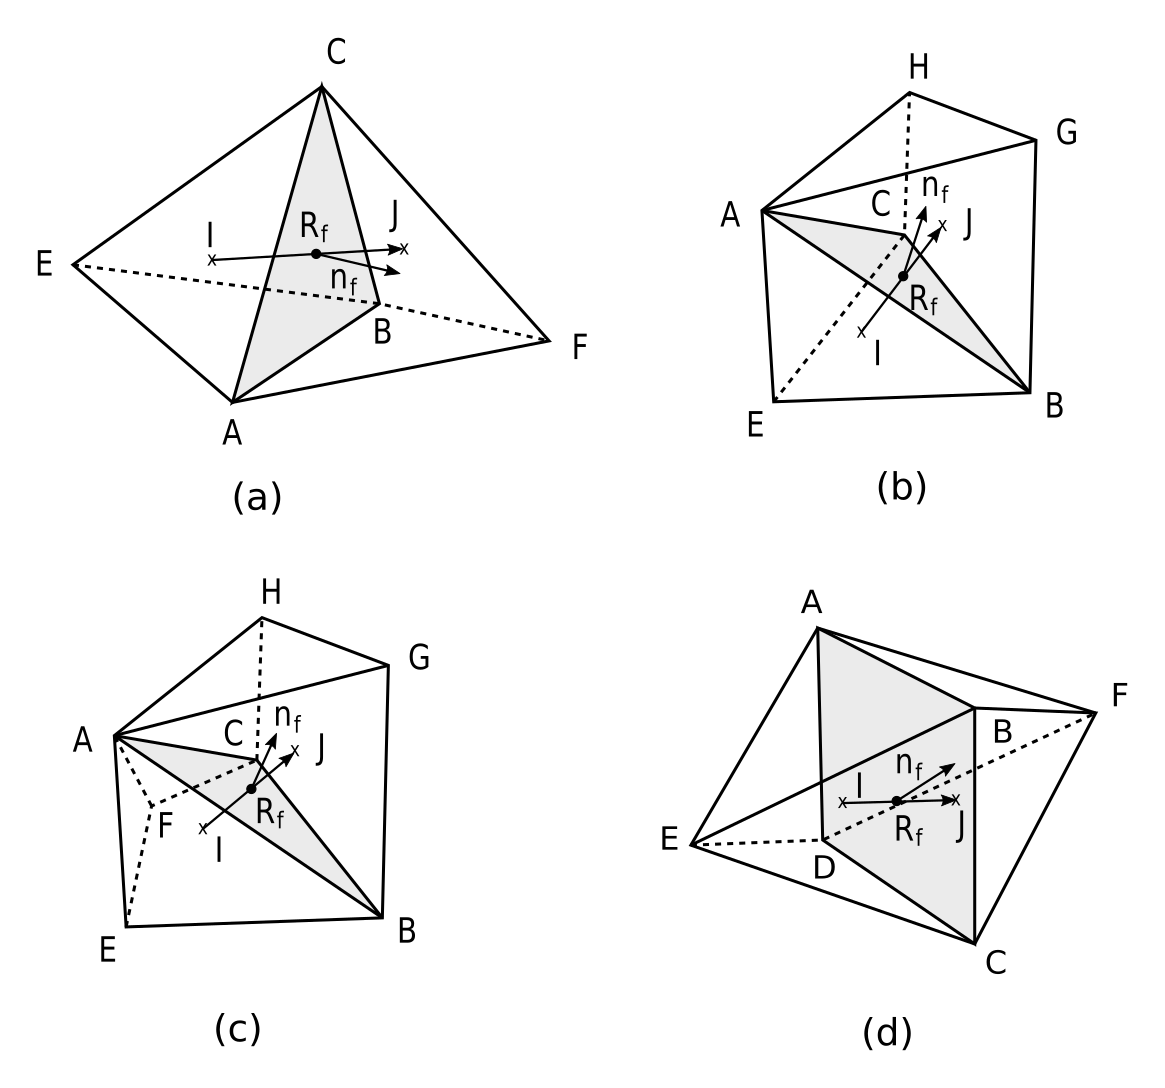
\includegraphics[width=0.9\textwidth]{figures/cases.png}
  \label{cases_figure}
  \caption{Example configuration in 2D and 3D. Note $A$, $B$ and $C$ can be arbitrary chosen}
\end{figure}



\subsection{Derivative of the objective function}

Using gradient base algorithm to solve the optimization problem (\ref{eq:opt_problem}) require the knowlegde of the objective function derivative relative to each point $P_i$ of coordinates $(x_i,y_i,z_i)$, which can expressed as the sum of the derivative of each individual face error $d E_f / dP_i$:
%
\begin{equation}
\frac{dc}{dP_i} = \sum_{f \in faces} \frac{d E_f}{d P_i}
\end{equation}
%
However, for a given mesh face $f$, if the two elements sharing the face $f$ do not contains the mesh point $P_i$, the derivative ${d E_f}{d P_i}$ will be null.
In fact, there is only few cases when the derivative is non-null, which can be grouped into three configurations (Figure X):
\begin{itemize}
\item the considered point is a face point (configuration $P_i = A$),
\item the considered point belong to the element pointed by the face normal (configuration $P_i = F$),
\item or the belong to the other element (configuration $P_i = E$).
\end{itemize}
%
The derivative of individual face error $E_f$ according to a mesh vertices $P$ could be therefore be simplified to read:
%
\begin{equation}
\frac{dE_f}{dP} = \sum_{f\in\ conf(P=A)} \frac{dE_f}{dA} + \sum_{f\in\ conf(P=E)} \frac{dE_f}{dE} +
\sum_{f\in\ conf(P=F)} \frac{dE_f}{dF} 
\end{equation}
%
where $f \in conf(P=X)$ states for the faces $f$ for which the point $P$ is in configuration $X$ (either $A$, $E$ or $F$, see Figure \ref{cases_figure}). 


\subsection{Individual face error derivative}

The general formula of the derivative of individual face error $E_f$ according to a mesh vertice $P_i$ is given by:
%
\begin{equation}
\frac{dE_f}{dP_i} = E'_f\left( r_f^T \cdot n_f, w_f \right) \left(n_f^T \cdot \frac{d r_f}{dP_i}\ +\ r_f^T \cdot \frac{d n_f}{dP_i}\right)
\label{general_derivative_expression}
\end{equation}
%
Where $E'_f$ is the weighting function derivative relative to its face orthogonality variable $(r_f^T \cdot n_f)$.
The evaluation of individual face error derivative (equation \ref{general_derivative_expression}) required the derivative of the face normal vector relative to the considered point $d n_f / dP_i$ and those of the cell center vector $d r_f / dP_i$, which are unit vector whose coordinates does not depend trivially on the mesh point $P_i$.
Expanding the unit vector derivative $du/dP_i$ to link it with its dimensional counterpart leads $dU/dP_i$ (see Annex A):
%
\begin{equation}
\frac{du}{dP_i} = \frac{1}{N} \left[ \boldsymbol{I} - \frac{1}{N^2}\ U \otimes U^T \right] \frac{dU}{dP_i}
\end{equation}
%
The previous formula to calculate the derivative of unit vector $n_f$ and $r_f$ relative to any mesh point $P_i$.
The previous formula could therefore be used to calculate 

Expression of the derviative for 3D tetrahedral and 2D quad and triangular mesh are provided in annexe.


\subsection{Numerical implementation}

A example implementation nammed OrthOpt is proposed at an online GitHub repository (\href{https://github.com/MoiseRousseau/Mesh-Orthogonality-Optimizer}{https://github.com/MoiseRousseau/Mesh-Orthogonality-Optimizer}) and uses the C++ programming language. 
This program takes as input the mesh to be optimized (in various format such as Medit or TetGen) and the optimization parameters.
The mesh is first decomposed, tetrahedron are stored and the internal connections are built. 
Optimization is then carried using a on-purpose class called OrthOpt which compute the objective function and the derivative according to vertice position. 
Finally, optimization is carried using the L-BFGS algorithm of the L-BGFSpp library \cite{} until a maximum number of iteration is reached.
The proposed implementation also benefits from the parallelization using OpenMP up to an arbitrary number of threads for the optimization process.
Input, output and mesh decomposition are, for instance, done in serial.

The constraint $r_f^T \cdot n_f \geq 0$ was imposed in the optimization by returning a NaN value when the dot product was negative, thus preventing the formation of inverted element.
%TODO speed up on girhub



\section{Application to simulation of diffusive problems}

\subsection{Test procedure}

This problem was solved numerically on a tetrahedral mesh with the OpenFOAM finite volume code \cite{} and using the LaplacianFoam application built-in application.
The reference, orthogonality-unoptimized mesh was generated using the open-source computer-aided design software Salome using the NETGEN algorithm \cite{schrobert_netgen}, and consisted in approximately 400~000 tetrahedra.
The Geometric Agglomerated Algebraic Multigrid (GAMG) solver combined with a Diagonal-based Incomplete Cholesky (DIC) smoother was used to solve the discretized set of equation. 
Relative and absolute tolerances were 1$\times$10\textsuperscript{-3} and 1$\times$10\textsuperscript{-6} respectively.

OpenFOAM relies on the TPFA method for discretization of the diffusion operator, which results in $\mathcal{O}(1)$ error on such tetrahedral mesh.
The iterative deferred correction approach implemented in OpenFOAM was also used to minimize the cross-diffusion error emerging from mesh non-orthogonality.
Therefore, the objective of this benchmark was (1) to assess the performance of the mesh orthogonality optimizer in terms of error relative to the true analytical solution of the Dirichlet BC - Laplacian ball, and (2) in terms of deffered correction convergence speed.
Multiple error function $E_f$ were considered and their influence on the performance of the mesh orthogonality optimizer are discussed below.
Several optimized meshes with different error function $E_f$ were considered to assess the influence of the error function on the performance of the optimization (see next paragraph).

The reference, NETGEN-generated mesh was next optimized using the proposed approach in this paper and using several different error function $E_f$.
In particular, a power function $E_f(x) = (1-x)^n$, an exponential function $E_f(x) = \exp \left[n(1-x) \right]$ and an inverse function $E_f(x) = 1/x^n$ were considered.
The $n$ parameter, called the penalization power, was also adapted to analyze further its influence on the final mesh.
For each mesh optimization, 200 L-BGFS iteration were carried.

Defered correction according to Jasak \cite{}. Performance according to convergence versus iteration.



\subsection{Two dimensional example}

\subsection{Three dimensional example}

The proposed methodology for mesh optimization was tested against solving the steady-state Laplace equation $\Delta u = 0$ in a ball of unit radius $a=1$ with a Dirichlet boundary condition applied at its surface $u(r,\theta,\phi) = F(\theta,\phi)$. %TODO
The previous Dirichlet BC - Laplacian ball problem possesses an analytical solution in the form of \cite{carslaw_jeager_1957}:
%
\begin{equation}
u(r, \theta, \phi) = \sum_{n=0}^\infty \sum_{m=0}^n \left(\frac{r}{a}\right)^n P_n^m(\cos \theta) \left[ A_{n,m} \cos m\phi + B_{n,m} \sin m\phi \right]
\end{equation} 
%
Where the $P_n$ are the Legendre polynomial of degree $n$, and $A_{n,m}$ and $B_{n,m}$ the coefficients such as:
%
\begin{equation}
F(\theta, \phi) = \sum_{n=0}^\infty \sum_{m=0}^n P_n^m(\cos \theta) \left[ A_{n,m} \cos m\phi + B_{n,m} \sin m\phi \right]
\end{equation}
%
In this benchmark problem, $A_{0,0} = A_{3,3} = B_{2,2} =1$ and all other coefficients were considered null.

A tetrahedral mesh was generated which have an average quality.
In the rest of this section, the distributions of the non-orthogonality angle in the optimized mesh were analyzed to compared the different error function and penalization power.
For the three function, the larger the penalization power $n$, the higher the penalization of the high non-orthogonality face is.
Considering first the exponential weighting function, distribution of the face non-orthogonality showed only slight modification of the distribution for a penalization power $n \leq 20$ (Figure \ref{orthogonality_distribution}a).

\begin{figure}[h!]
  \centering
  \includegraphics[width=0.99\textwidth]{simulation/sphere/mesh_compare/mesh_compare.pdf}
  \label{orthogonality_distribution}
  \caption{Distribution of face non-orthogonality in the optimized meshes considering (a) an exponential weighting function, (b) a power weighting function and (c) an inverse function for various penalization power $n$. The black curve the reference, unoptimized mesh generated with the NETGEN algorithm.}
\end{figure}



\subsection{Comparing Numerical and Analytical Solutions}





\section{Discussion}

In all the cases simulated, decrease of error without correction and decrease of GAMG iteration. 
So no counterproductive results were obtain.
User may used this everytimes

\subsection{Influence of Penalization Function}

Choosing the right function $E_f$ is critical to ensure both a effective mesh orthogonality optimization and the creation of non-inverted elements. 
For example, choosing $E_f$ as a power law function (i.e. $E_f=w_f (1-r_f^T\cdot n_f)^n$) with a penalization power $n=5$ would decrease the mean non orthogonality of the mesh.
At the opposite, a high penalization power (e.g. $n=5$) would preferentially decreases the non-orthogonality of internal faces with a high error.


\subsection{Conductive and Diffusive Problems}

Influence on mesh skewness

\subsection{Discussion}

Cell of a prisms not considered. Tet and pyramid are optimized. Cell must be either hexa, pyr or tet.
%TODO say we are optimizing point belonging to triangle, not quad, because of an additional equality constraint

Anisotropy can't work.
Unless grid are K orthogonal \cite{heinemann_modelling_1991}.
However, no possible for tetrahedron

Conventional two-point flux approximation (TPFA) can only obtain the flux normal to the grid interface but completely neglects the one parallel to it \cite{}. MPFA needed. %https://ui.adsabs.harvard.edu/abs/2017AGUFM.H31D1541L/abstract

Inverted element.

Further work.
2D case.
Weighting factor as a function of the configuration.
Include skewness error for gradient operator


\section{Conclusion}

TODO



\bibliography{references.bib}
\bibliographystyle{apalike}


\clearpage


\section*{Annex: Derivative of the objective function}

\subsection*{A. Unit vector derivative relative to a point}
Starting from the definition of a unit vector $u$:
\begin{equation}
u = \frac{U}{N}
\end{equation}
With $U$ a non unit vector and $N$ its norm.
Derivate according to a particular point $X$ write:
\begin{equation}
\frac{du}{dX} = \frac{1}{N^2} \left[ N \frac{dU}{dX} - U \otimes \frac{dN}{dX} \right]
\end{equation}
Where the sign $\otimes$ represent the dyadic product. Derivative of the vector norm $N$ expresses:
\begin{equation}
\frac{dN}{dX} = \frac{d}{dX} \sqrt{\sum_i U_i^2} =
\frac{1}{N} \sum_i U_i \frac{dU_i}{dX}
\end{equation}
Which simplifies to:
\begin{equation}
\frac{dN}{dX} = \frac{1}{N}\ U^T \frac{dU}{dX}
\end{equation}
Replacing the above expression in those of the derivative of the unit vector $u$ leads, after dyatic product rearangement and factorization:
\begin{equation}
\frac{du}{dX} = \frac{1}{N} \left[ \boldsymbol{I} - u \otimes u^T \right] \frac{dU}{dX} = \frac{1}{N} \left[ \boldsymbol{I} - \frac{1}{N^2}\ U \otimes U^T \right] \frac{dU}{dX}
\end{equation}
With $\boldsymbol{I}$ the unit 3x3 diagonal matrix.


\subsection*{B. Expressions of cell center vectors and their derivative}

\subsubsection*{Case 1}

Center of a tetrahedra is given by the arithmetic mean of its four vertices:
\begin{subequations}
\begin{gather}
I = \frac{1}{4} (A + B + C + E) \\
J = \frac{1}{4} (A + B + C + F)
\end{gather}
\end{subequations} 
Therefore, cell center vector $R_f$ reads:
\begin{equation}
R_f = \| r_f \|\ r_f = J-I = \frac{1}{4} (F - E)
\end{equation}
Which permitted to express the derivative of $R_f$ according to a mesh vertice $P$ depending if $P$ is either $A$, $E$ or $F$:
\begin{subequations}
\begin{align}
\frac{d R_f}{d A} &= \ 0 \\
\frac{d R_f}{d F} &= - \frac{d R_f}{d E} = \frac{1}{4}\ \boldsymbol{I}
\end{align}
\end{subequations} 

\subsubsection*{Case 2}

In the second case, the center of the tetrahedra $I$ and of the pyramid $J$ are given by:
\begin{subequations}
\begin{gather}
I = \frac{1}{4} (A + B + C + E) \\
J = \frac{A}{4} + \frac{1}{16} (B + C + G + H)
\end{gather}
\end{subequations} 
Therefore, cell center vector $R_f$ reads:
\begin{equation}
R_f = J-I = -\frac{E}{4} - \frac{3}{16} (B + C) + \frac{1}{16} ( G + H)
\end{equation}
In this case, only the $A$ and $E$ point are non fixed. Derivative of the cell center vector according to these two points is thus:
\begin{subequations}
\begin{align}
\frac{d R_f}{d A} &= \ 0 \\
\frac{d R_f}{d E} &= - \frac{1}{4}\ \boldsymbol{I}
\end{align}
\end{subequations}


\subsubsection*{Case 3}

Center of both pyramids are given by:
\begin{subequations}
\begin{gather}
I = \frac{A}{4} + \frac{1}{16} (B + C + K + L) \\
J = \frac{A}{4} + \frac{1}{16} (B + C + G + H)
\end{gather}
\end{subequations} 
Cell center vector $R_f$ reads:
\begin{equation}
R_f = \frac{1}{16} ( G + H - K - L)
\end{equation}
In this case, only point $A$ is non fixed, which therefore give:
\begin{equation}
\frac{d R_f}{d A} = \ 0 
\end{equation}


\subsubsection*{Case 4}

Center of both pyramids are given by:
\begin{subequations}
\begin{gather}
I = \frac{E}{4} + \frac{1}{16} (A + B + C + D) \\
J = \frac{F}{4} + \frac{1}{16} (A + B + C + D)
\end{gather}
\end{subequations} 
Cell center vector $R_f$ reads:
\begin{equation}
R_f = \frac{1}{4} (F-E)
\end{equation}
And derivative is:
\begin{equation}
\frac{d R_f}{d F} = - \frac{d R_f}{d E} = \frac{1}{4}\ \boldsymbol{I}
\end{equation}



\subsection*{C. Expressions of the derivatives}

\subsubsection*{Unit cell center vector term}

Derivative of the unit cell center vector $r_f$ according to a point $P$ write (see Annex A):
\begin{equation}
\frac{d r_f}{dP}\ = 
- \frac{1}{\| R_f \|} \left[ \boldsymbol{I} - r_f \otimes r_f^T \right] \frac{d R_f}{dP}
\end{equation}
Also, the cell center vector derivative is either 0 for $P$ in position $A$, $\boldsymbol{I} /4$ if $P$ is in position $F$ or the opposite if in position $E$ (if non fixed, see Annex B). 
Therefore, the term implying the unit cell center vector in Eq. (\ref{general_derivative_expression}) write:
\begin{equation}
n_f^T\ \frac{d r_f}{dF}\ = - n_f^T\ \frac{d r_f}{dE} =
 \frac{1}{4 \| R_f \|} \left[n_f^T- n_f^T \cdot (r_f \otimes r_f^T) \right]
\end{equation}
Rearranging the parentesis finally lead to the general expression of the unit cell center vector derivative:
\begin{subequations}
\begin{align}
n_f^T\ \frac{d r_f}{dA}\ &=  0 \\
n_f^T\ \frac{d r_f}{dE}\ &= - \frac{1}{4 \| R_f \|} \left[ n_f^T - (n_f^T \cdot r_f)\ r_f^T \right] \\
n_f^T\ \frac{d r_f}{dF}\ &=  \frac{1}{4 \| R_f \|} \left[ n_f^T - (n_f^T \cdot r_f)\  r_f^T \right]
\end{align}
\end{subequations} 



\end{document}